\documentclass[12pt,a4paper]{article}

% ── Core packages ──────────────────────────────────────────────────
\usepackage[utf8]{inputenc}
\usepackage[T1]{fontenc}
\usepackage[english]{babel}
\usepackage{lmodern}

% ── Math ──────────────────────────────────────────────────────────
\usepackage{amsmath,amsfonts,amssymb}

% ── Layout ────────────────────────────────────────────────────────
\usepackage{geometry}
\geometry{a4paper, left=30mm, right=25mm, top=30mm, bottom=30mm}
\usepackage{setspace}
\setstretch{1.2}
\usepackage{parskip}
\setlength{\parindent}{0pt}
\setlength{\parskip}{6pt}

% ── Tables ────────────────────────────────────────────────────────
\usepackage{array,booktabs,longtable,multirow,tabularx,multicol}
\usepackage{caption}
\captionsetup{font=small,labelfont=bf}

% ── Graphics & Diagrams ───────────────────────────────────────────
\usepackage{graphicx}
\graphicspath{{./assets/}}
\usepackage{float}
\usepackage{tikz}
\usetikzlibrary{arrows.meta,positioning,fit,calc,shapes.geometric,backgrounds}

% ── Colors ────────────────────────────────────────────────────────
\usepackage{xcolor}
\definecolor{titlebg}{RGB}{25,55,100}
\definecolor{sectioncolor}{RGB}{25,55,100}
\definecolor{accentblue}{RGB}{0,90,160}
\definecolor{codebg}{HTML}{F5F5F5}
\definecolor{codeframe}{HTML}{CCCCCC}
\definecolor{codecomment}{HTML}{6A9955}
\definecolor{codekeyword}{HTML}{0055AA}
\definecolor{codestring}{HTML}{A31515}
\definecolor{alertbg}{RGB}{255,248,220}
\definecolor{successbg}{RGB}{242,255,242}
\definecolor{infobg}{RGB}{240,248,255}
\definecolor{dkgreen}{rgb}{0,0.6,0}
\definecolor{gray}{rgb}{0.5,0.5,0.5}

% ── Section formatting ────────────────────────────────────────────
\usepackage{titlesec}
\titleformat{\section}
  {\Large\bfseries\color{sectioncolor}}
  {\Roman{section}.}{0.7em}{}[\color{sectioncolor}\titlerule]
\titleformat{\subsection}
  {\large\bfseries\color{sectioncolor!85}}
  {\thesubsection}{0.7em}{}
\titleformat{\subsubsection}
  {\normalsize\bfseries\color{sectioncolor!70}}
  {\thesubsubsection}{0.7em}{}
\setcounter{secnumdepth}{3}

% ── Header / Footer ───────────────────────────────────────────────
\usepackage{fancyhdr}
\usepackage{lastpage}
\pagestyle{fancy}
\fancyhf{}
\fancyhead[L]{\small\textit{DIMT — Document Intelligent Machine Translation}}
\fancyhead[R]{\small\thepage/\pageref{LastPage}}
\renewcommand{\headrulewidth}{0.4pt}
\renewcommand{\footrulewidth}{0pt}

% ── Hyperlinks ────────────────────────────────────────────────────
\usepackage{hyperref}
\hypersetup{
  colorlinks=true,
  linkcolor=accentblue,
  citecolor=accentblue,
  urlcolor=accentblue,
  pdftitle={DIMT Pipeline Report},
}

% ── Listings (code blocks) ────────────────────────────────────────
\usepackage{listings}
\lstset{
  backgroundcolor=\color{codebg},
  basicstyle=\ttfamily\small,
  breaklines=true,
  captionpos=b,
  commentstyle=\color{codecomment}\itshape,
  frame=single,
  framerule=0.4pt,
  rulecolor=\color{codeframe},
  keywordstyle=\color{codekeyword}\bfseries,
  stringstyle=\color{codestring},
  numberstyle=\tiny\color{gray},
  numbers=left,
  numbersep=8pt,
  showstringspaces=false,
  tabsize=2,
  xleftmargin=12pt,
  xrightmargin=4pt,
}
\lstdefinelanguage{JSONL}{
  morestring=[b]",
  stringstyle=\color{codestring},
  literate={:}{{{\color{accentblue}:}}}1
            {,}{{{\color{gray},}}}1,
}

% ── Misc ──────────────────────────────────────────────────────────
\usepackage{mdframed}
\usepackage{enumitem}
\setlist[itemize]{noitemsep, topsep=3pt}
\setlist[enumerate]{noitemsep, topsep=3pt}

% ── Callout boxes ─────────────────────────────────────────────────
\newmdenv[
  linecolor=accentblue!60,
  backgroundcolor=infobg,
  roundcorner=4pt,
  skipabove=8pt,
  skipbelow=8pt,
  innerleftmargin=10pt,
  innerrightmargin=10pt,
  innertopmargin=6pt,
  innerbottommargin=6pt
]{infobox}

\newmdenv[
  linecolor=dkgreen!60,
  backgroundcolor=successbg,
  roundcorner=4pt,
  skipabove=8pt,
  skipbelow=8pt,
  innerleftmargin=10pt,
  innerrightmargin=10pt
]{successbox}

% ─────────────────────────────────────────────────────────────────
\begin{document}

% ═══════════════════════════════════════════════════════════════════
%  TITLE PAGE
% ═══════════════════════════════════════════════════════════════════
\begin{titlepage}
\thispagestyle{empty}
\begin{center}

{\large VIETNAM NATIONAL UNIVERSITY HO CHI MINH CITY}\\[4pt]
{\large\bfseries UNIVERSITY OF SCIENCE}\\[4pt]
{\normalsize Faculty of Information Technology}

\vspace{1.5cm}

\begin{tikzpicture}
  \node[draw=sectioncolor, line width=2pt, rounded corners=6pt,
        fill=white, inner sep=12pt] {
    \begin{tabular}{c}
      \includegraphics[width=3.5cm]{khtn.jpg}
    \end{tabular}
  };
\end{tikzpicture}

\vspace{1.5cm}

{\color{sectioncolor}\rule{\textwidth}{1.5pt}}\\[8pt]
{\huge\bfseries\color{sectioncolor} DIMT}\\[6pt]
{\Large\bfseries Document Intelligent Machine Translation}\\[6pt]
{\large\color{gray} NLP Pipeline — Technical Report}\\[8pt]
{\color{sectioncolor}\rule{\textwidth}{1.5pt}}

\vspace{1.8cm}

\begin{tabular}{rl}
  \textbf{Lecturers:}  & Nguyen Hong Buu Long \\
                       & Luong An Vinh \\[8pt]
  \textbf{Students:}   & Nguyen Dang Minh Duy \quad 23127042 \\
                       & Thieu Quang Vinh \quad\quad\ 23127143 \\
                       & Luong Thanh Loc \quad\quad\ 23127405 \\
\end{tabular}

\vfill

{\footnotesize Ho Chi Minh City, May 2026}

\end{center}
\end{titlepage}

% ═══════════════════════════════════════════════════════════════════
%  TABLE OF CONTENTS
% ═══════════════════════════════════════════════════════════════════
\tableofcontents
\newpage

% ═══════════════════════════════════════════════════════════════════
\section{Business Problem Definition}
% ═══════════════════════════════════════════════════════════════════

\subsection{Business Context and Motivation}

Scientific papers and technical documents are routinely distributed in PDF format, combining complex layouts with text, figures, tables, diagrams, and mathematical notation. Universities, research groups, publishers, and multinational companies continuously need these documents translated into multiple languages to support international collaboration and knowledge sharing.

Manual translation followed by document reformatting is laborious and expensive. Existing translation tools focus on plain text and do not preserve the original visual structure, causing a loss of readability and formatting consistency that is particularly harmful in scientific and technical content. There is therefore a clear need for an automated, end-to-end pipeline that can both translate document content and faithfully reconstruct the original page layout.

\subsection{Target Users and Stakeholders}

The system is designed for:

\begin{itemize}
  \item Students and researchers accessing foreign-language scientific materials.
  \item Academic institutions and digital libraries.
  \item Scientific publishers and conference organizers.
  \item International organizations requiring multilingual technical documentation.
\end{itemize}

Key stakeholders include end users who need translated documents, research institutions aiming to improve document accessibility, and organizations seeking to reduce manual translation costs and processing time.

\subsection{Problem Description}

DIMT (\emph{Document Intelligent Machine Translation}) is an end-to-end multilingual document translation pipeline targeting PDF-based scientific documents.

The system accepts a PDF document as input, extracts textual content, layout structure, and bounding-box coordinates, translates the extracted text into target languages (German and French) using neural machine translation models, and renders the translated content back into the original document layout. The final output is a translated PDF that preserves both the semantic meaning and the visual structure of the original.

\subsection{Why NLP is Required}

Natural Language Processing is essential because the system must understand and translate human language automatically while preserving contextual meaning. Traditional rule-based approaches are insufficient for scientific terminology and multilingual text.

The Neural Machine Translation models used — MarianMT and NLLB — enable context-aware translation, multilingual support, better handling of scientific terminology, and higher fluency compared to conventional methods. Without NLP techniques the system could not provide scalable and accurate multilingual document translation.

% ─────────────────────────────────────────────────────────────────
% Overall pipeline diagram
% ─────────────────────────────────────────────────────────────────
\begin{figure}[H]
\centering
\resizebox{0.96\columnwidth}{!}{%
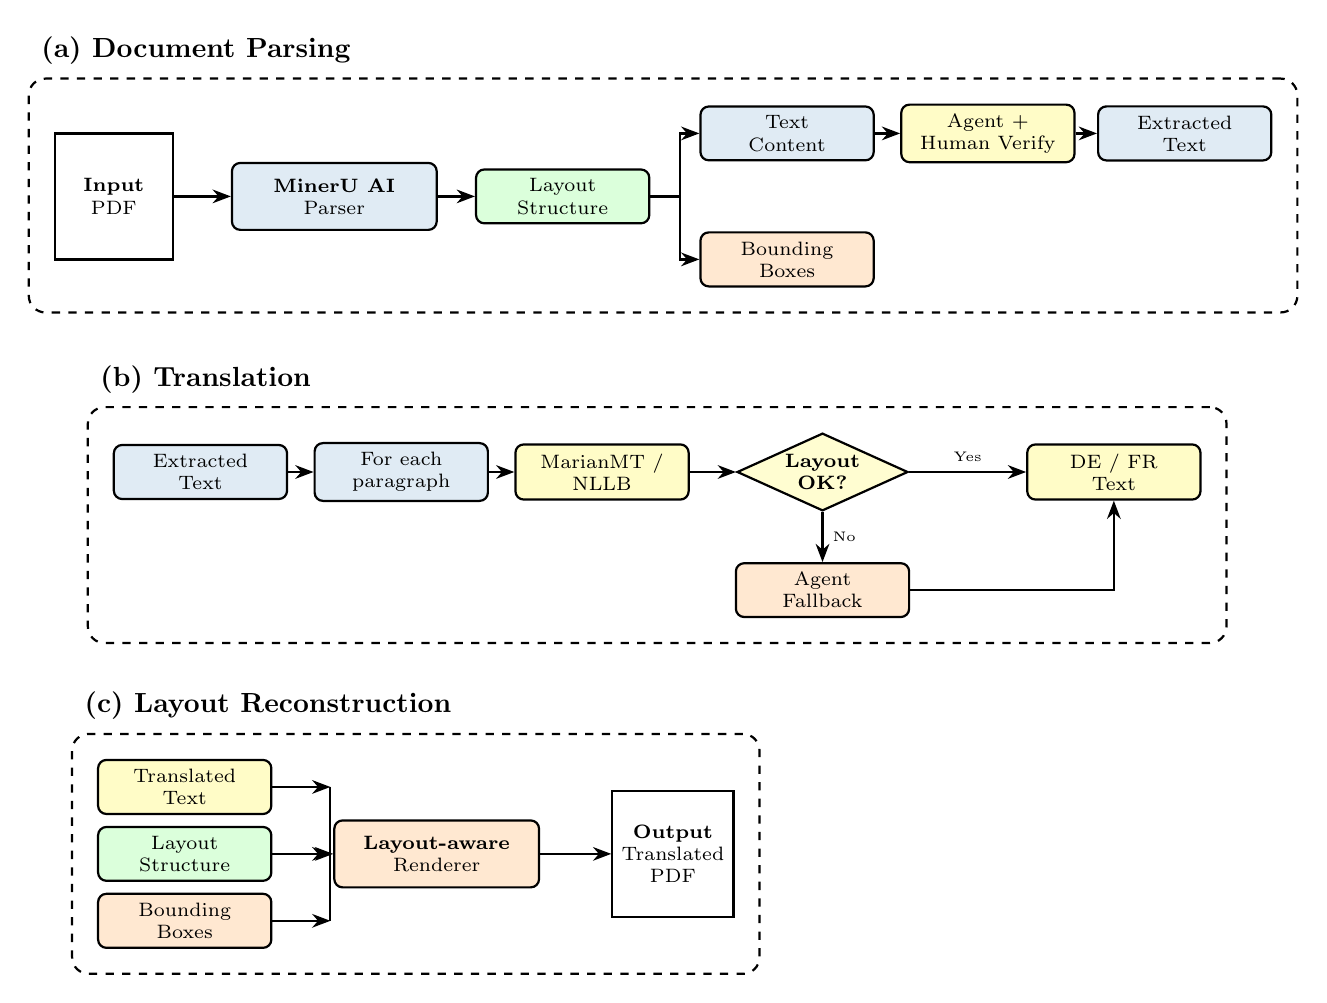
\begin{tikzpicture}[
    font=\scriptsize,
    >=Stealth,
    arrow/.style={->, thick},
    block/.style={draw, rounded corners=3pt, thick, minimum width=2.6cm,
                  minimum height=0.85cm, align=center, fill=white},
    smallblock/.style={draw, rounded corners=3pt, thick, minimum width=2.2cm,
                       minimum height=0.65cm, align=center, fill=white},
    decision/.style={draw, diamond, thick, aspect=2.2, inner sep=1pt,
                     align=center, fill=yellow!18},
    doc/.style={draw, thick, minimum width=1.5cm, minimum height=1.6cm,
                align=center, fill=white},
    group/.style={draw, dashed, thick, rounded corners=6pt, inner sep=9pt},
    parse/.style={fill=accentblue!12},
    translate/.style={fill=yellow!22},
    layout/.style={fill=green!14},
    render/.style={fill=orange!18},
]

%% ── (a) Document Parsing ──────────────────────────────────────
\node[doc]                  (pdf)    at (0,1.25)    {\textbf{Input}\\PDF};
\node[block,parse]          (mineru) at (2.8,1.25)  {\textbf{MinerU AI}\\Parser};
\node[smallblock,layout]    (struct) at (5.7,1.25)  {Layout\\Structure};
\node[smallblock,parse]     (text)   at (8.55,2.05) {Text\\Content};
\node[smallblock,render]    (bbox)   at (8.55,0.45) {Bounding\\Boxes};
\node[smallblock,translate] (verify) at (11.1,2.05) {Agent +\\Human Verify};
\node[smallblock,parse]     (xtxt)   at (13.6,2.05) {Extracted\\Text};

\draw[arrow] (pdf)    -- (mineru);
\draw[arrow] (mineru) -- (struct);
\draw[arrow] (struct.east) -- ++(0.38,0) |- (text.west);
\draw[arrow] (struct.east) -- ++(0.38,0) |- (bbox.west);
\draw[arrow] (text)   -- (verify);
\draw[arrow] (verify) -- (xtxt);

\node[group, fit=(pdf)(mineru)(struct)(text)(bbox)(verify)(xtxt)] (ga) {};
\node[font=\bfseries, anchor=south west] at ($(ga.north west)+(0.05,0.04)$)
  {(a) Document Parsing};

%% ── (b) Translation ──────────────────────────────────────────
\node[smallblock,parse]     (tin)   at (1.1,-2.25)  {Extracted\\Text};
\node[smallblock,parse]     (fep)   at (3.65,-2.25) {For each\\paragraph};
\node[smallblock,translate] (mdls)  at (6.2,-2.25)  {MarianMT /\\NLLB};
\node[decision]             (chk)   at (9.0,-2.25)  {\textbf{Layout}\\\textbf{OK?}};
\node[smallblock,translate] (tout)  at (12.7,-2.25) {DE / FR\\Text};
\node[smallblock,render]    (agnt)  at (9.0,-3.75)  {Agent\\Fallback};

\draw[arrow] (tin)  -- (fep);
\draw[arrow] (fep)  -- (mdls);
\draw[arrow] (mdls) -- (chk);
\draw[arrow] (chk.east) -- node[above,font=\tiny]{Yes} (tout.west);
\draw[arrow] (chk.south) -- node[right,font=\tiny]{No} (agnt.north);
\draw[arrow] (agnt.east) -- ++(1.4,0) -| (tout.south);

\node[group, fit=(tin)(fep)(mdls)(chk)(tout)(agnt)] (gb) {};
\node[font=\bfseries, anchor=south west] at ($(gb.north west)+(0.05,0.04)$)
  {(b) Translation};

%% ── (c) Layout Reconstruction ────────────────────────────────
\node[smallblock,translate] (trtxt)  at (0.9,-6.25)  {Translated\\Text};
\node[smallblock,layout]    (lmeta)  at (0.9,-7.10)  {Layout\\Structure};
\node[smallblock,render]    (bmeta)  at (0.9,-7.95)  {Bounding\\Boxes};
\node[block,render]         (rend)   at (4.1,-7.10)  {\textbf{Layout-aware}\\Renderer};
\node[doc]                  (opdf)   at (7.1,-7.10)  {\textbf{Output}\\Translated\\PDF};

\coordinate (bus0) at (2.75,-6.25);
\coordinate (bus1) at (2.75,-7.10);
\coordinate (bus2) at (2.75,-7.95);
\draw[thick] (bus0) -- (bus2);
\draw[arrow] (trtxt.east) -- (bus0);
\draw[arrow] (lmeta.east) -- (bus1);
\draw[arrow] (bmeta.east) -- (bus2);
\draw[arrow] (bus1)  -- (rend.west);
\draw[arrow] (rend)  -- (opdf);

\node[group, fit=(trtxt)(lmeta)(bmeta)(rend)(opdf)] (gc) {};
\node[font=\bfseries, anchor=south west] at ($(gc.north west)+(0.05,0.04)$)
  {(c) Layout Reconstruction};

\end{tikzpicture}
}
\caption{DIMT pipeline grouped into three stages: document parsing, neural translation, and layout-aware PDF reconstruction.}
\label{fig:pipeline}
\end{figure}

% ═══════════════════════════════════════════════════════════════════
\section{Dataset Overview}
% ═══════════════════════════════════════════════════════════════════

DoTA (\emph{Document Image Machine Translation Dataset of arXiv articles}) provides document images together with MultiMarkdown transcriptions and translations of scientific papers. Within this workspace the text-side \texttt{.mmd} files are used rather than the image files.

The original repository describes DoTA as a dataset for document image machine translation, with English source files and translated Chinese, French, and German \texttt{.mmd} files. The local processing pipeline adapts that material into a plain-text parallel corpus suitable for NLLB-200 fine-tuning.

\begin{table}[H]
\centering
\caption{Main DoTA directories and files used by the local JSONL preparation pipeline.}
\label{tab:dota-layout}
\renewcommand{\arraystretch}{1.25}
\begin{tabularx}{\linewidth}{lX}
\toprule
\textbf{Directory / File} & \textbf{Role in this workspace} \\
\midrule
\texttt{en\_mmd/}                        & English source MultiMarkdown files; file name is the join key. \\
\texttt{fr\_mmd/}                        & French target files paired with \texttt{en\_mmd} by identical name. \\
\texttt{de\_mmd/}                        & German target files paired with \texttt{en\_mmd} by identical name. \\
\texttt{Dataset/train.jsonl}             & Training split generated from cleaned source–target pairs. \\
\texttt{Dataset/test.jsonl}              & Held-out test split. \\
\texttt{Dataset/val.jsonl}               & Validation split. \\
\texttt{build\_dataset.py}               & Main orchestration script: reads \texttt{.mmd} files, writes JSONL. \\
\texttt{Processing/text\_cleaner.py}     & Text normalization and quality-filtering module. \\
\bottomrule
\end{tabularx}
\end{table}

% ═══════════════════════════════════════════════════════════════════
\section{Why Convert \texttt{.mmd} to JSONL for NLLB}
% ═══════════════════════════════════════════════════════════════════

NLLB fine-tuning expects text pairs in a machine-readable structure. The raw DoTA \texttt{.mmd} files contain Markdown headings, links, tables, LaTeX math, citations, and other markup that can harm a translation model if treated as ordinary natural language.

\begin{itemize}
  \item JSONL stores one training example per line — compatible with Hugging Face \texttt{datasets} and streaming readers.
  \item Each record holds a source string, a target string, and the NLLB target language code.
  \item Paragraph-level alignment keeps examples long enough to preserve context but short enough for efficient fine-tuning.
  \item Cleaning removes document-formatting artifacts so the model focuses on translation rather than markup reconstruction.
\end{itemize}

% ═══════════════════════════════════════════════════════════════════
\section{Output JSONL Schema}
% ═══════════════════════════════════════════════════════════════════

The pipeline writes one JSON object per line:

\begin{lstlisting}[language=JSONL, caption={JSONL record format.}]
{"source": "English cleaned paragraph",
 "target": "Translated cleaned paragraph",
 "tgt_lang": "fra_Latn|deu_Latn"}
\end{lstlisting}

\begin{table}[H]
\centering
\caption{JSONL fields produced by the active DoTA preprocessing pipeline.}
\label{tab:jsonl-schema}
\renewcommand{\arraystretch}{1.25}
\begin{tabularx}{\linewidth}{llX}
\toprule
\textbf{Field} & \textbf{Meaning} & \textbf{Example} \\
\midrule
\texttt{source}   & Cleaned English text from \texttt{en\_mmd}. & \textit{This method improves the posterior estimate.} \\
\texttt{target}   & Cleaned translated text from target \texttt{.mmd}. & \textit{Cette méthode améliore l'estimation\ldots} \\
\texttt{tgt\_lang} & NLLB target language code. & \texttt{fra\_Latn} or \texttt{deu\_Latn} \\
\bottomrule
\end{tabularx}
\end{table}

% ═══════════════════════════════════════════════════════════════════
\section{The Two Python Files Used by the Pipeline}
% ═══════════════════════════════════════════════════════════════════

\begin{table}[H]
\centering
\caption{Python files used to convert DoTA \texttt{.mmd} files into NLLB-ready JSONL.}
\label{tab:python-files}
\renewcommand{\arraystretch}{1.25}
\begin{tabularx}{\linewidth}{lXl}
\toprule
\textbf{File} & \textbf{Primary responsibility} & \textbf{Key functions} \\
\midrule
\texttt{build\_dataset.py} & Coordinates the dataset build and writes JSONL. &
  \makecell[l]{\texttt{collect\_pairs}\\ \texttt{split\_with\_unique\_sources}\\ \texttt{write\_jsonl}\\ \texttt{assert\_no\_overlap}\\ \texttt{main}} \\
\addlinespace
\texttt{Processing/text\_cleaner.py} & Cleans and filters \texttt{.mmd} text before training. &
  \makecell[l]{\texttt{clean\_markdown}\\ \texttt{split\_paragraphs}\\ \texttt{is\_valid\_sentence}\\ \texttt{normalize\_whitespace}\\ \texttt{strip\_latex\_environments}} \\
\bottomrule
\end{tabularx}
\end{table}

% ═══════════════════════════════════════════════════════════════════
\section{\texttt{build\_dataset.py}: End-to-End Orchestration}
% ═══════════════════════════════════════════════════════════════════

The main script turns document-level parallel \texttt{.mmd} files into record-level JSONL examples, using file names as alignment keys.

\subsection{Configuration}

\begin{table}[H]
\centering
\caption{Important configuration values in \texttt{build\_dataset.py}.}
\label{tab:build-config}
\renewcommand{\arraystretch}{1.25}
\begin{tabularx}{\linewidth}{llX}
\toprule
\textbf{Setting} & \textbf{Value} & \textbf{Purpose} \\
\midrule
\texttt{EN\_DIR}             & \texttt{ROOT/en\_mmd}          & Source language directory. \\
\texttt{LANG\_PAIRS}         & \texttt{fr\_mmd/fra\_Latn}, \texttt{de\_mmd/deu\_Latn} & Supported target languages. \\
\texttt{DEFAULT\_MAX\_PAIRS} & 15\,000 per language pair      & Caps the number of retained records. \\
\texttt{DEFAULT\_OUTPUT\_DIR}& \texttt{ROOT/Dataset}          & Output directory for JSONL splits. \\
\texttt{DEFAULT\_SEED}       & 42                             & Reproducible shuffling and splitting. \\
Split ratios                 & 0.90 / 0.05 / 0.05             & Train / test / validation. \\
\bottomrule
\end{tabularx}
\end{table}

\subsection{Collection Logic}

The \texttt{collect\_pairs} function is the core reader. It lists all English \texttt{.mmd} files, shuffles them with the configured seed, and iterates until every target language has reached the requested quota or source files are exhausted.

\begin{enumerate}
  \item Read an English \texttt{.mmd} file from \texttt{en\_mmd} using UTF-8 with error tolerance.
  \item Split the English document into paragraphs with \texttt{split\_paragraphs}.
  \item For each configured language pair, locate a target \texttt{.mmd} file with the same name.
  \item Read and split the target file into paragraphs.
  \item Skip the target file when paragraph counts differ, because paragraph-level alignment is no longer reliable.
  \item For each aligned paragraph pair, call \texttt{clean\_markdown} on both sides.
  \item Reject either side when \texttt{is\_valid\_sentence} flags it as too short, too long, too symbol-heavy, or still contaminated by markup.
  \item Deduplicate by cleaned English source text within each language pair.
  \item Append a record with \texttt{source}, \texttt{target}, and \texttt{tgt\_lang}.
\end{enumerate}

\subsection{Splitting Without Source Leakage}

\texttt{split\_with\_unique\_sources} prevents the same English source paragraph from appearing in both training and evaluation data. It groups all records by the \texttt{source} field, shuffles the unique source keys, then assigns whole groups to train, test, or validation.

The split is performed over unique source groups, not individual rows. Therefore, if an English paragraph has both French and German translations, all translations of that paragraph stay in the same split.

\subsection{JSONL Writing}

After collecting and splitting records, \texttt{write\_jsonl} creates the output directory if needed and writes each Python dictionary as one UTF-8 JSON object per line, using \texttt{ensure\_ascii=False} so multilingual target text is preserved directly.

\begin{lstlisting}[language=bash, caption={CLI usage examples for \texttt{build\_dataset.py}.}]
python build_dataset.py
python build_dataset.py --max-pairs-per-lang 15000 --seed 42
python build_dataset.py --output-dir Dataset \
                        --train-ratio 0.9 \
                        --test-ratio 0.05 \
                        --val-ratio 0.05
\end{lstlisting}

% ═══════════════════════════════════════════════════════════════════
\section{\texttt{Processing/text\_cleaner.py}: Cleaning and Filtering}
% ═══════════════════════════════════════════════════════════════════

The cleaner module is deliberately separate from the build script, keeping text normalization reusable and independently testable.

\subsection{\texttt{split\_paragraphs}}

Divides a document on blank lines. A paragraph is kept only if it contains non-whitespace text after stripping.

\subsection{\texttt{clean\_markdown}}

Performs ordered normalization. The order matters because many markup forms are nested: LaTeX environments are removed first, before smaller regex passes handle residual syntax.

\begin{table}[H]
\centering
\caption{Ordered cleaning stages implemented by \texttt{clean\_markdown}.}
\label{tab:clean-stages}
\renewcommand{\arraystretch}{1.25}
\begin{tabularx}{\linewidth}{lX}
\toprule
\textbf{Stage} & \textbf{What it removes or transforms} \\
\midrule
Unicode normalization  & Normalizes text to NFC for stable regex behavior. \\
LaTeX environments     & Removes complete \texttt{begin/end} blocks (tabular, align, equation, figure, …). \\
Code                   & Removes fenced code blocks and inline code. \\
Images, links, URLs    & Drops images and bare URLs; keeps visible link text. \\
Math                   & Removes block and inline math delimiters and content. \\
LaTeX commands         & Removes remaining commands, escapes, orphan delimiters, tabular column specs. \\
Markdown blocks        & Removes table lines, rules, headings, blockquotes, list markers. \\
Emphasis               & Strips bold and italic markers, preserving inner text. \\
HTML, footnotes, citations & Removes tags, footnote markers, numeric citations. \\
Whitespace             & Collapses spaces and blank lines; fixes spacing around punctuation. \\
\bottomrule
\end{tabularx}
\end{table}

\subsection{\texttt{strip\_latex\_environments}}

Removes full LaTeX environment blocks, including nested environments of the same type. If a \texttt{\textbackslash begin} tag has no matching \texttt{\textbackslash end}, only the opening tag is removed — a conservative behavior that avoids accidentally deleting large document sections due to malformed markup.

\subsection{\texttt{is\_valid\_sentence}}

Applies quality filters after cleaning to reject weak training examples.

\begin{table}[H]
\centering
\caption{Quality filters applied by \texttt{is\_valid\_sentence}.}
\label{tab:valid-sent}
\renewcommand{\arraystretch}{1.25}
\begin{tabularx}{\linewidth}{llX}
\toprule
\textbf{Check} & \textbf{Default threshold} & \textbf{Reason} \\
\midrule
Length               & 10–1500 chars              & Avoids fragments and very long noisy blocks. \\
Letter count         & $\geq 5$ letters           & Rejects mostly numeric or symbolic content. \\
Letter ratio         & $\geq 0.4$                 & Keeps natural-language-heavy examples. \\
Tabular residue      & $\leq 2$ ampersand sep.    & Removes leftover table fragments. \\
LaTeX escapes        & None                       & Avoids teaching escaped markup as language. \\
Orphan math delims   & None                       & Rejects partially cleaned math markup. \\
Header markers       & None                       & Rejects remaining Markdown headings. \\
\bottomrule
\end{tabularx}
\end{table}

% ═══════════════════════════════════════════════════════════════════
\section{Full Pipeline Flow}
% ═══════════════════════════════════════════════════════════════════

\begin{enumerate}
  \item Start with parallel \texttt{.mmd} directories: \texttt{en\_mmd} and one or more target-language directories.
  \item Run \texttt{build\_dataset.py} from the repository root.
  \item The script imports \texttt{clean\_markdown}, \texttt{split\_paragraphs}, and \texttt{is\_valid\_sentence} from \texttt{Processing/text\_cleaner.py}.
  \item English source files are discovered, shuffled, and read.
  \item Target files are matched by identical file name.
  \item Source and target documents are split by blank-line paragraph boundaries.
  \item Misaligned files (different paragraph counts) are skipped.
  \item Each paragraph pair is cleaned and quality-filtered.
  \item Records are capped and deduplicated per language pair.
  \item All language-pair records are merged.
  \item Records are grouped by source text and split into train / test / validation without source overlap.
  \item The final JSONL files are written under \texttt{Dataset/}.
\end{enumerate}

% ═══════════════════════════════════════════════════════════════════
\section{Current Local Output}
% ═══════════════════════════════════════════════════════════════════

\begin{table}[H]
\centering
\caption{Current local JSONL split sizes.}
\label{tab:local-output}
\renewcommand{\arraystretch}{1.25}
\begin{tabular}{lrl}
\toprule
\textbf{File} & \textbf{Lines} & \textbf{Use} \\
\midrule
\texttt{Dataset/train.jsonl} & 27\,001 & Training examples. \\
\texttt{Dataset/test.jsonl}  &  1\,501 & Held-out test examples. \\
\texttt{Dataset/val.jsonl}   &  1\,498 & Validation examples. \\
\midrule
\textbf{Total}               & 30\,000 & \\
\bottomrule
\end{tabular}
\end{table}

% ═══════════════════════════════════════════════════════════════════
\section{Using the JSONL Files for NLLB Fine-Tuning}
% ═══════════════════════════════════════════════════════════════════

The JSONL files can be consumed directly by Hugging Face \texttt{datasets}:

\begin{lstlisting}[language=Python, caption={Loading the dataset splits with Hugging Face.}]
from datasets import load_dataset

data_files = {
    "train":      "Dataset/train.jsonl",
    "validation": "Dataset/val.jsonl",
    "test":       "Dataset/test.jsonl",
}

dataset = load_dataset("json", data_files=data_files)
print(dataset["train"][0])
\end{lstlisting}

\begin{infobox}
\textbf{Training configuration notes:}
\begin{itemize}
  \item Source language is always English: \texttt{eng\_Latn}.
  \item Target language is read per row from \texttt{tgt\_lang} (\texttt{fra\_Latn} or \texttt{deu\_Latn}).
  \item The tokenizer must be configured consistently with the model's language-code handling.
  \item Evaluation should be run on \texttt{test.jsonl}; validation guides model selection or early stopping.
\end{itemize}
\end{infobox}

% ═══════════════════════════════════════════════════════════════════
\section{Operational Notes and Caveats}
% ═══════════════════════════════════════════════════════════════════

\begin{itemize}
  \item The active dataset builder covers EN-FR and EN-DE only. \texttt{zh\_mmd} and \texttt{vi\_mmd} are not currently included.
  \item Paragraph count mismatch causes a target file to be skipped — this favors correctness over volume.
  \item The cleaner removes most math, tables, and document structure. This is appropriate for plain-text translation fine-tuning but not for layout-preserving document translation.
  \item Deduplication occurs per language pair during collection; split leakage prevention is applied globally by source after all records are merged.
  \item The repository also contains \texttt{Processing/prepare\_chunked\_json.py} — a separate EN-VI pipeline that writes only \texttt{train.jsonl} and \texttt{test.jsonl}. It is not the active three-split pipeline described here.
\end{itemize}

% ═══════════════════════════════════════════════════════════════════
\section{Practical Rebuild Checklist}
% ═══════════════════════════════════════════════════════════════════

\begin{enumerate}
  \item Confirm \texttt{en\_mmd}, \texttt{fr\_mmd}, and \texttt{de\_mmd} exist and contain matching \texttt{.mmd} file names.
  \item Run \texttt{python build\_dataset.py} from the repository root.
  \item Review the printed collection statistics for missing files, read errors, misalignment, invalid sentences, and duplicates.
  \item Confirm \texttt{Dataset/train.jsonl}, \texttt{Dataset/test.jsonl}, and \texttt{Dataset/val.jsonl} were updated.
  \item Inspect a few random rows for encoding, language codes, and source-target alignment.
  \item Run downstream training or validation scripts against the generated \texttt{Dataset} directory.
\end{enumerate}

% ═══════════════════════════════════════════════════════════════════
\section{Source Files Referenced}
% ═══════════════════════════════════════════════════════════════════

\begin{table}[H]
\centering
\caption{Source files referenced in this report.}
\label{tab:source-files}
\renewcommand{\arraystretch}{1.25}
\begin{tabularx}{\linewidth}{lX}
\toprule
\textbf{Path} & \textbf{Reason it matters} \\
\midrule
\texttt{build\_dataset.py}              & Main JSONL dataset construction script. \\
\texttt{Processing/text\_cleaner.py}    & Cleaner and validation module imported by \texttt{build\_dataset.py}. \\
\texttt{README.md}                      & Dataset background and citation information from the local DoTA repository. \\
\texttt{src/backend/nllb\_service.py}   & Production NLLB translation service; shows how the fine-tuned model is consumed. \\
\texttt{src/backend/marianmt\_service.py} & MarianMT translation service; alternative NMT backend. \\
\texttt{config/inference.yaml}          & Model paths and generation hyperparameters for both NMT backends. \\
\bottomrule
\end{tabularx}
\end{table}

\end{document}
